\documentclass{../../slides-style}

\slidetitleext[Часть 2]{Лекция 7: Управление проектами, планирование и управление}{02.04.2024}{Управление проектами}

\begin{document}

    \begin{frame}[plain]
        \titlepage
    \end{frame}

    \section{Планирование проекта}

    \begin{frame}
        \frametitle{Хороший график работ}
        \begin{itemize}
            \item Основывается на детальной декомпозиции
            \item Содержит все задачи в правильном порядке
            \item Учитывает сторонние ограничения (за пределами команды)
            \item Может быть завершён вовремя при наличии нужных ресурсов
            \item Направлен на достижение целей проекта
        \end{itemize}
    \end{frame}

    \begin{frame}
        \frametitle{Планирование проекта}
        \begin{enumerate}
            \item Определение сути проекта
            \item Разработка стратегии управления рисками
            \item Декомпозиция проекта
            \item Выявление зависимостей между задачами
            \item Оценка задач
            \item Создание и оценка плана работ
            \item Распределение и оптимизация ресурсов
        \end{enumerate}
    \end{frame}

    \begin{frame}
        \frametitle{Матрица зависимостей}
        \begin{center}
            \begin{tabularx}{\textwidth} { 
                | >{\centering\arraybackslash}X 
                | >{\centering\arraybackslash}X 
                | >{\centering\arraybackslash}X | }
                \hline
                Операция                                  & Непосредственно предшествующие операции & Длительность \\
                \hline
                A. Установка компьютеров                  & ---                                     & 1            \\
                \hline
                B. Протяжка сети                          & ---                                     & 2            \\
                \hline
                C. Настройка сети                         & A, B                                    & 3            \\
                \hline
                D. Установка программного обеспечения     & C                                       & 1            \\
                \hline
                E. Разработка регламента использования ПО & ---                                     & 4            \\
                \hline
                F. Обучение пользователей                 & D, E                                    & 3            \\
                \hline
            \end{tabularx}
        \end{center}
    \end{frame}

    \begin{frame}
        \frametitle{Сетевой график}
        \begin{center}
            \begin{tikzpicture}
                [every path/.style={font=\ssmall}]

                \node[shape=circle,draw=black] (1) at (0,0) {1};
                \node[shape=circle,draw=black] (2) at (2.5,1.5) {2};
                \node[shape=circle,draw=black] (3) at (2.5,-1.5) {3};
                \node[shape=circle,draw=black] (4) at (5,0) {4};
                \node[shape=circle,draw=black] (5) at (8,0) {5};
                \node[shape=circle,draw=black] (6) at (11,0) {6} ;
                
                \path [->](1) edge node[align=center] {A. Установка компьютеров\\ \textit{1 день}} (2);
                \path [->](1) edge node[align=center] {B. Протяжка сети\\ \textit{2 дня}} (3);
                \path [->,dashed](3) edge node[] {} (2);
                \path [->](2) edge node[align=center] {C. Настройка сети\\ \textit{1 день}} (4);
                \path [->](4) edge node[align=center,below=5pt] {D. Установка программного\\ обеспечения\\ \textit{1 день}} (5);
                \path [->](5) edge node[align=center,below=5pt] {F. Обучение\\ пользователей\\ \textit{1 день}} (6);
                \path [->](1) edge[bend right=70] node[align=center,below] {E. Разработка регламента\\использования ПО\\ \textit{1 день}} (5);
            \end{tikzpicture}
        \end{center}
    \end{frame}

    \section{Оценка задач}

    \begin{frame}
        \frametitle{Оценка задач}
        \begin{enumerate}
            \item Длительность
            \begin{itemize}
                \item Календарное время от начала работ до получения конечного результата
                \item Часы, дни, ...
            \end{itemize}
            \item Объём работ
            \begin{itemize}
                \item Абстрактные единицы работы для решения задачи
                \item Человеко-часы, человеко-дни, ...
            \end{itemize}
            \item Конвертация одного в другое
        \end{enumerate}

        $$\textup{Длительность работ} = \frac{\textup{Объём работ}}{\textup{Производительность}}$$
    \end{frame}

    \begin{frame}
        \frametitle{Чем занимаются программисты, когда пишут код}
        \begin{center}
            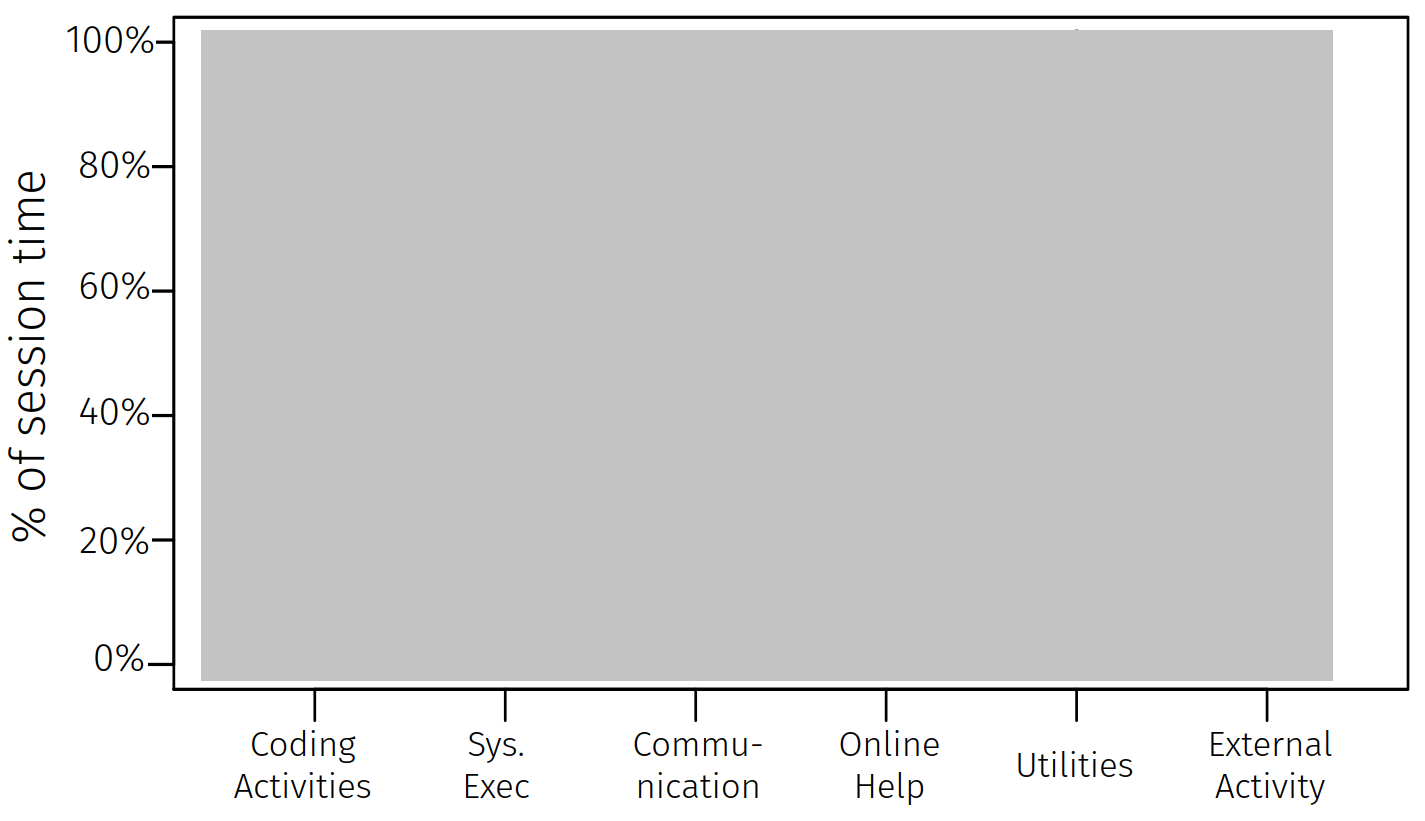
\includegraphics[width=0.95\textwidth]{timeSpentDuringWorkingSessionBlurred.png}
            \attribution{Astromskis et al. Patterns of Developers Behaviour: A 1,000-hour Industrial Study, 2017}
        \end{center}
    \end{frame}

    \begin{frame}
        \frametitle{Чем занимаются программисты, когда пишут код}
        \begin{center}
            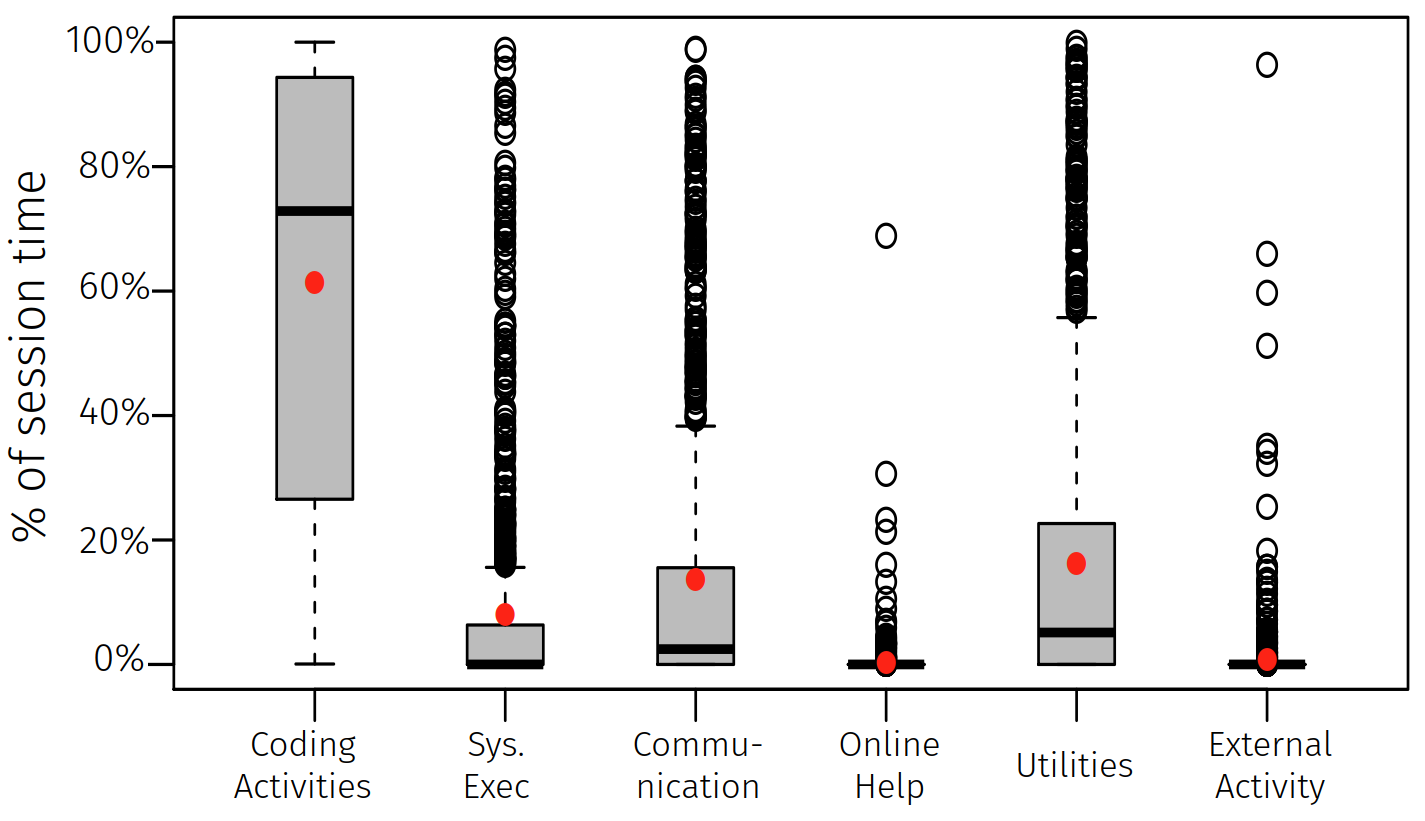
\includegraphics[width=0.95\textwidth]{timeSpentDuringWorkingSession.png}
            \attribution{Astromskis et al. Patterns of Developers Behaviour: A 1,000-hour Industrial Study, 2017}
        \end{center}
    \end{frame}

    \begin{frame}
        \frametitle{Чем занимаются программисты на работе вообще}
        \begin{center}
            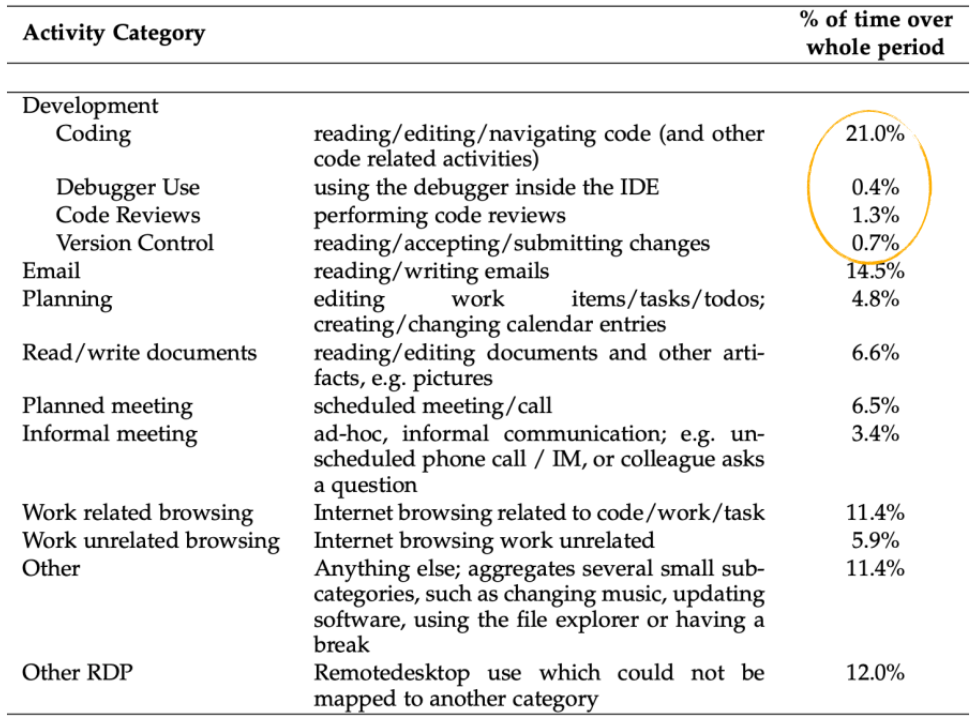
\includegraphics[width=0.7\textwidth]{timeSpentTotal.png}
            \attribution{Meyer et al. The work life of developers: Activities, switches and perceived productivity, 2017}
        \end{center}
    \end{frame}

    \begin{frame}
        \frametitle{Оценка графика работ}
        \begin{itemize}
            \item Прямой проход
            \item Обратный проход
            \item Вычисление резервов
            \item Критический путь
        \end{itemize}
        \begin{center}
            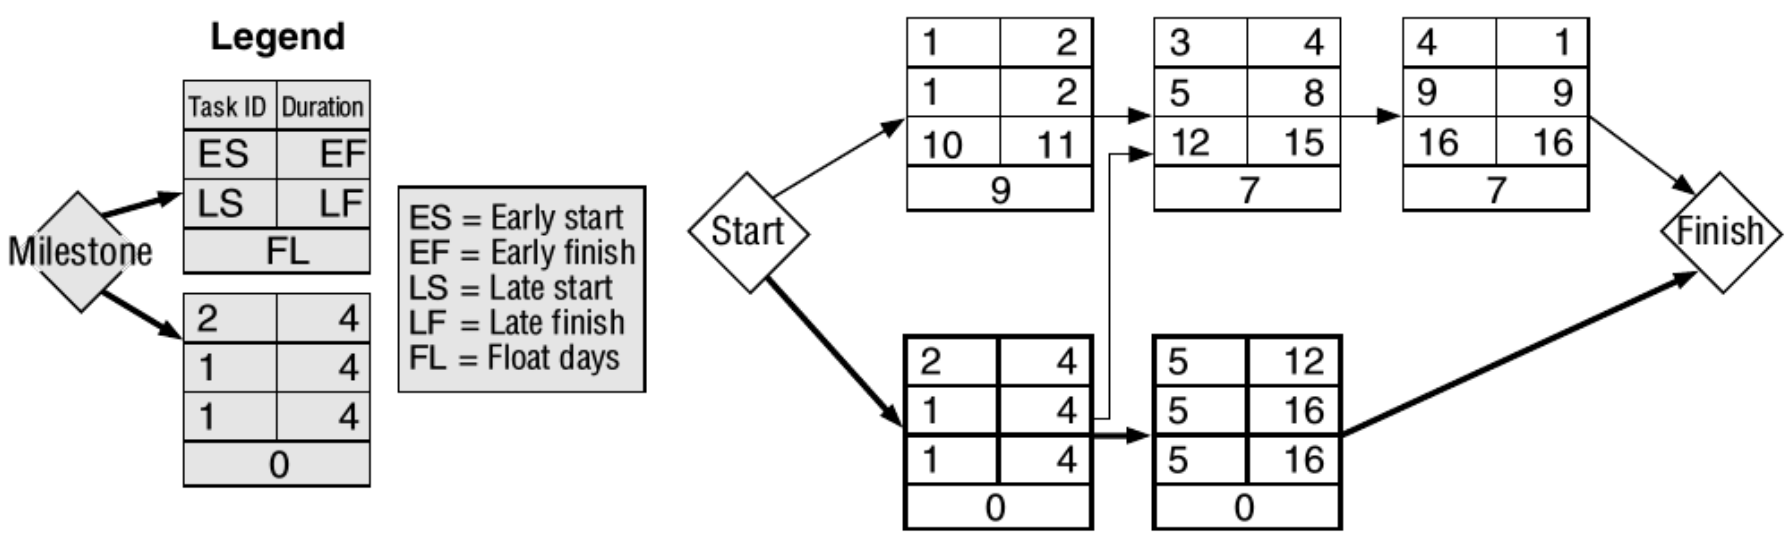
\includegraphics[width=0.95\textwidth]{graphEstimate.png}
        \end{center}
    \end{frame}

    \section{Календарный график}

    \begin{frame}
        \frametitle{Другой формат представления графика}
        \begin{center}
            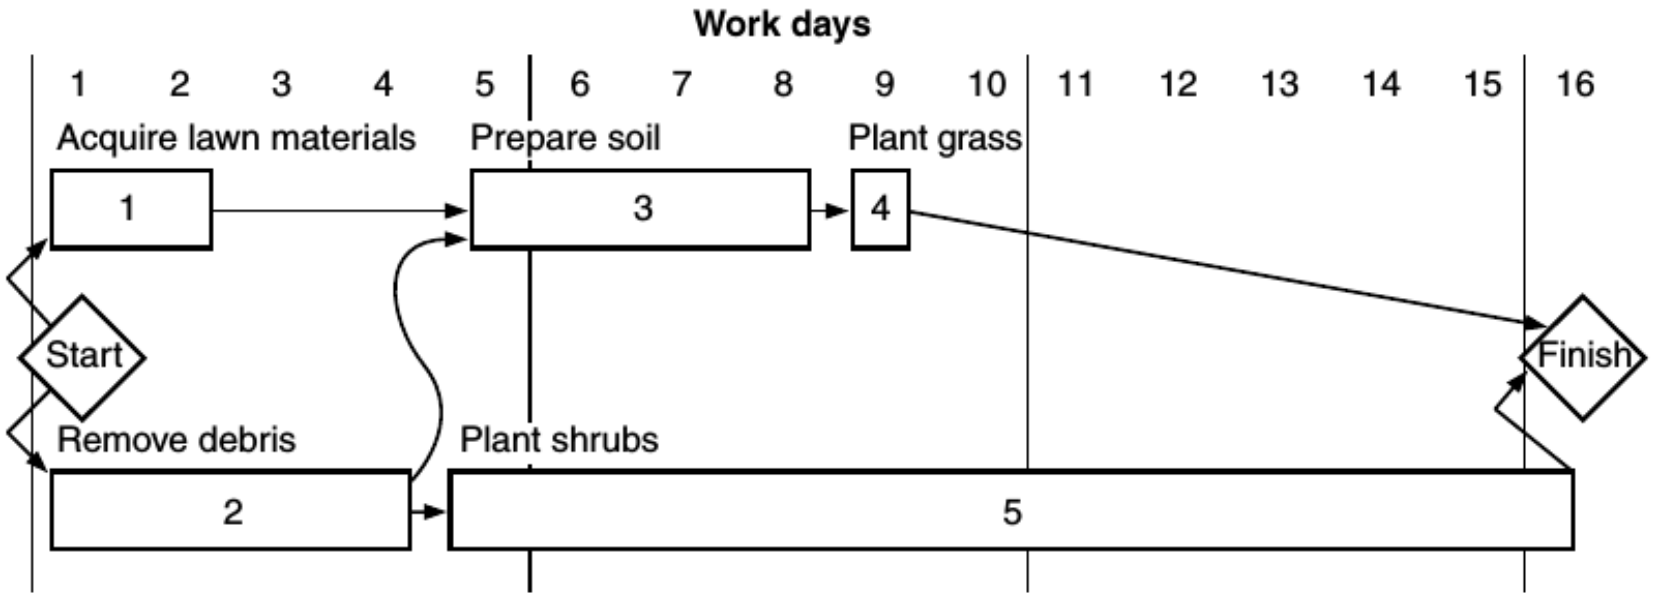
\includegraphics[width=0.95\textwidth]{otherGraphFormat.png}
        \end{center}
    \end{frame}

    \begin{frame}
        \frametitle{Диаграмма Гантта}
        \begin{itemize}
            \item 1910 год!
            \item Календарный график + зависимости работ
            \item Early start
        \end{itemize}
        \begin{center}
            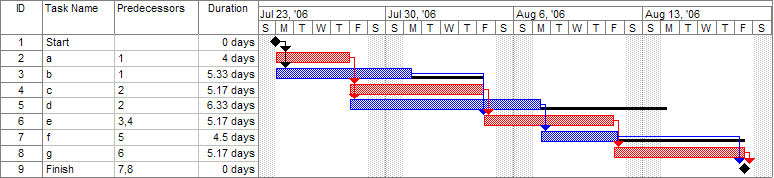
\includegraphics[width=0.95\textwidth]{ganttChart.png}
        \end{center}
    \end{frame}

    \begin{frame}
        \frametitle{Диаграмма Гантта, пример}
        \begin{center}
            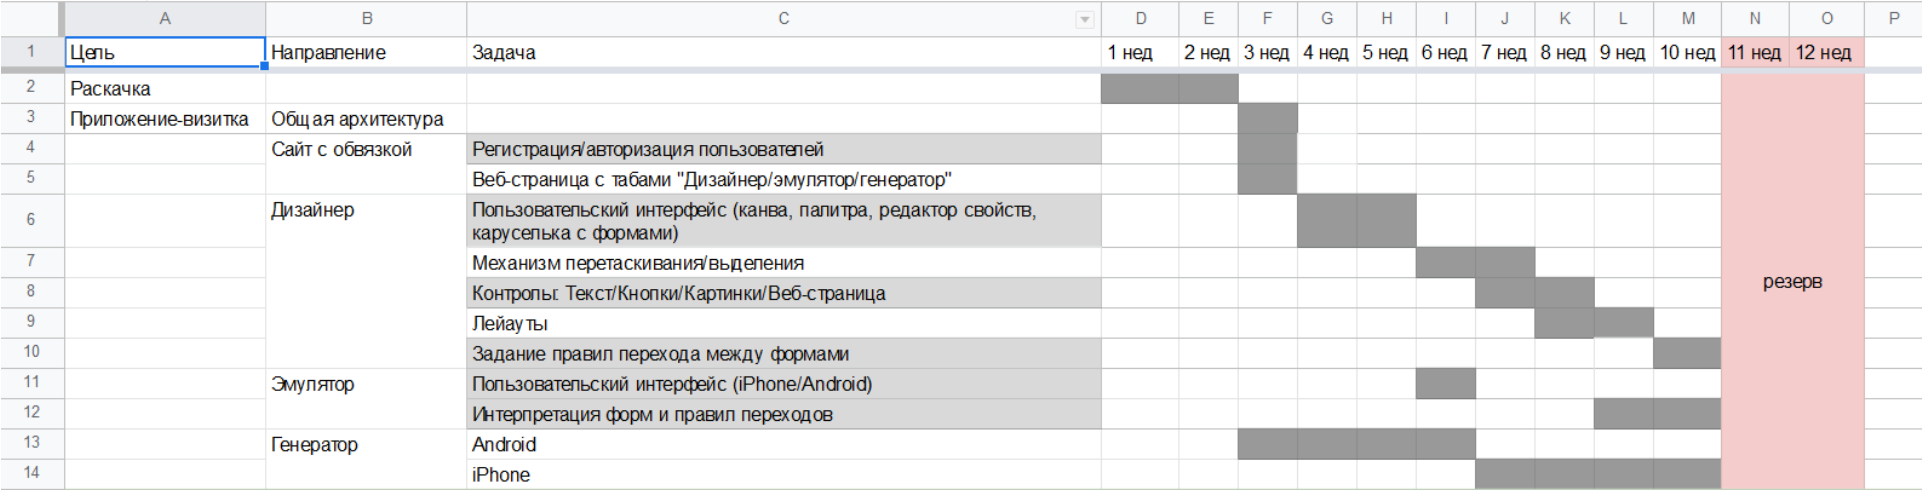
\includegraphics[width=0.95\textwidth]{ganttChartExample.png}
        \end{center}
    \end{frame}

    \begin{frame}
        \frametitle{Диаграмма Гантта с ресурсами}
        \begin{center}
            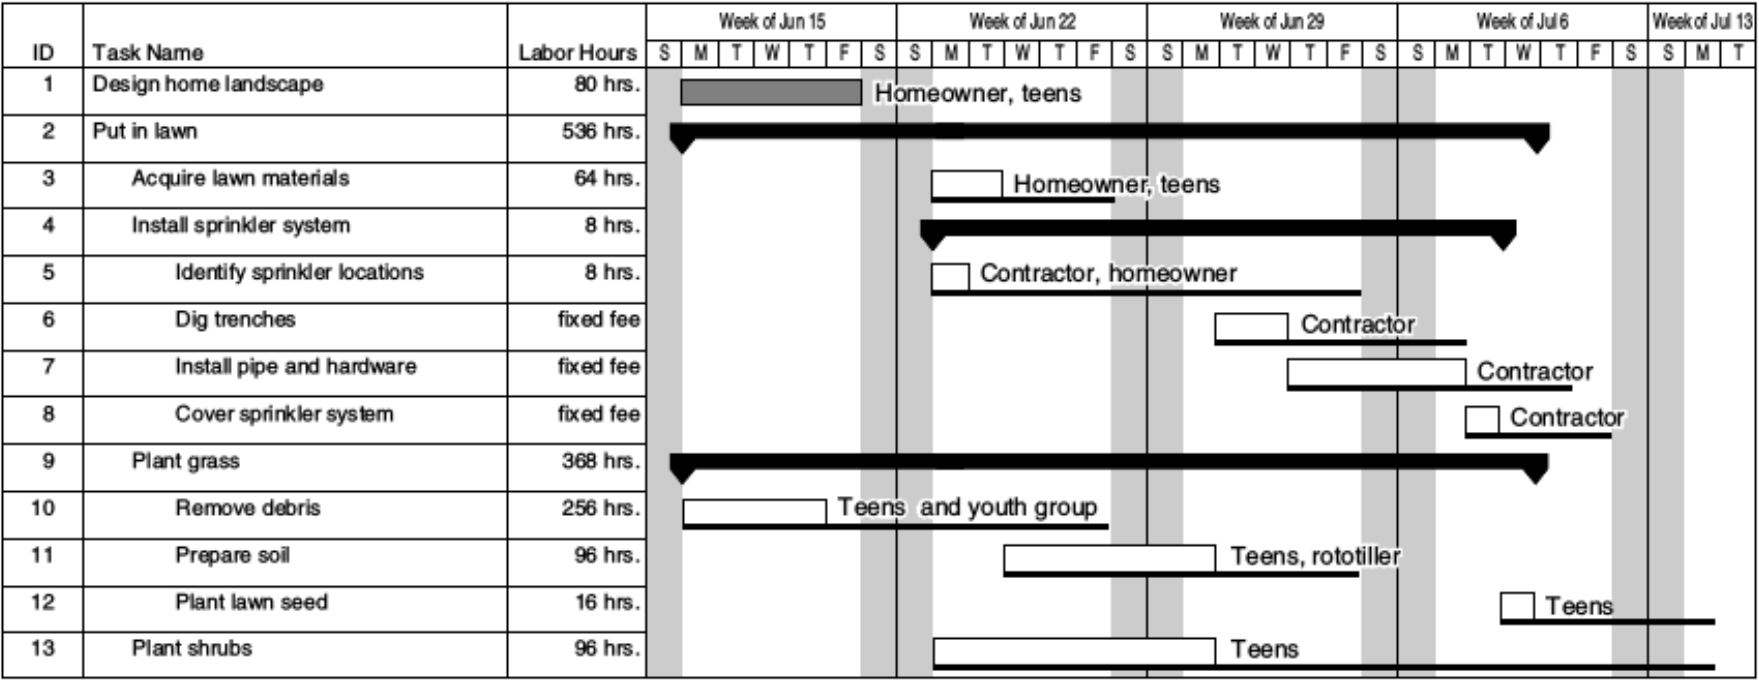
\includegraphics[width=0.95\textwidth]{ganttChartWithResources.png}
        \end{center}
    \end{frame}

    \begin{frame}
        \frametitle{Загруженность ресурсов}
        \begin{center}
            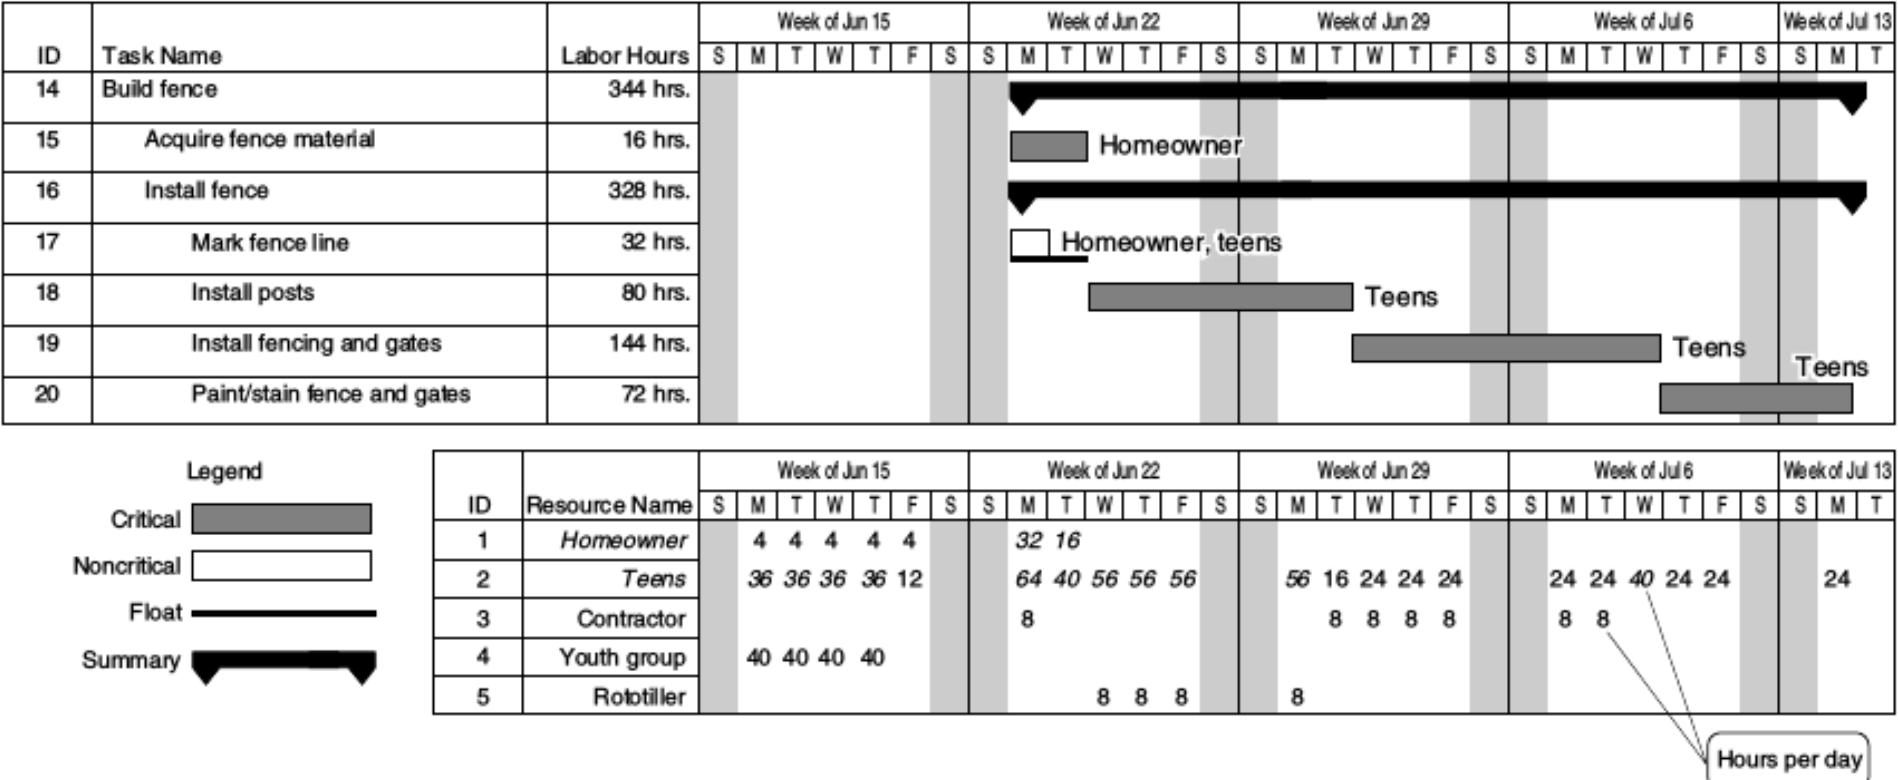
\includegraphics[width=0.95\textwidth]{ganttChartResourceUtilization.png}
        \end{center}
    \end{frame}

    \begin{frame}
        \frametitle{Оптимизация ресурсов}
        \begin{itemize}
            \item Перегруженность и недозагруженность
            \item Оценка ресурсов по начальному графику
            \item Определение и выравнивание пиков
            \item Переоценка задач, перераспределение людей
        \end{itemize}
        \begin{center}
            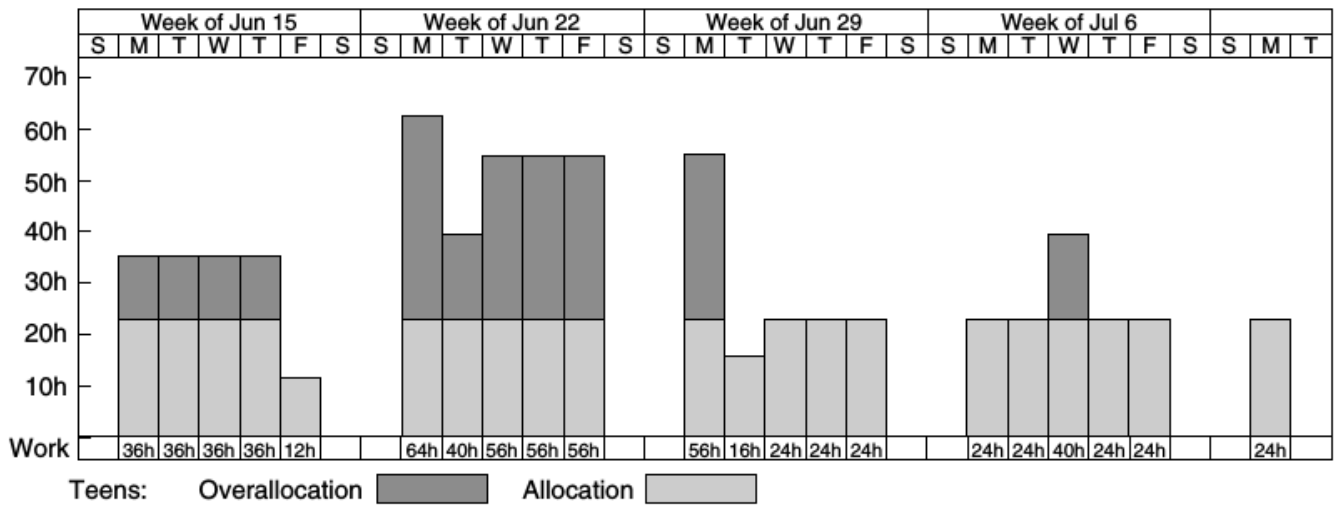
\includegraphics[width=0.7\textwidth]{resourceAllocation.png}
        \end{center}
    \end{frame}

    \begin{frame}
        \frametitle{Планирование денежного потока}
        \begin{center}
            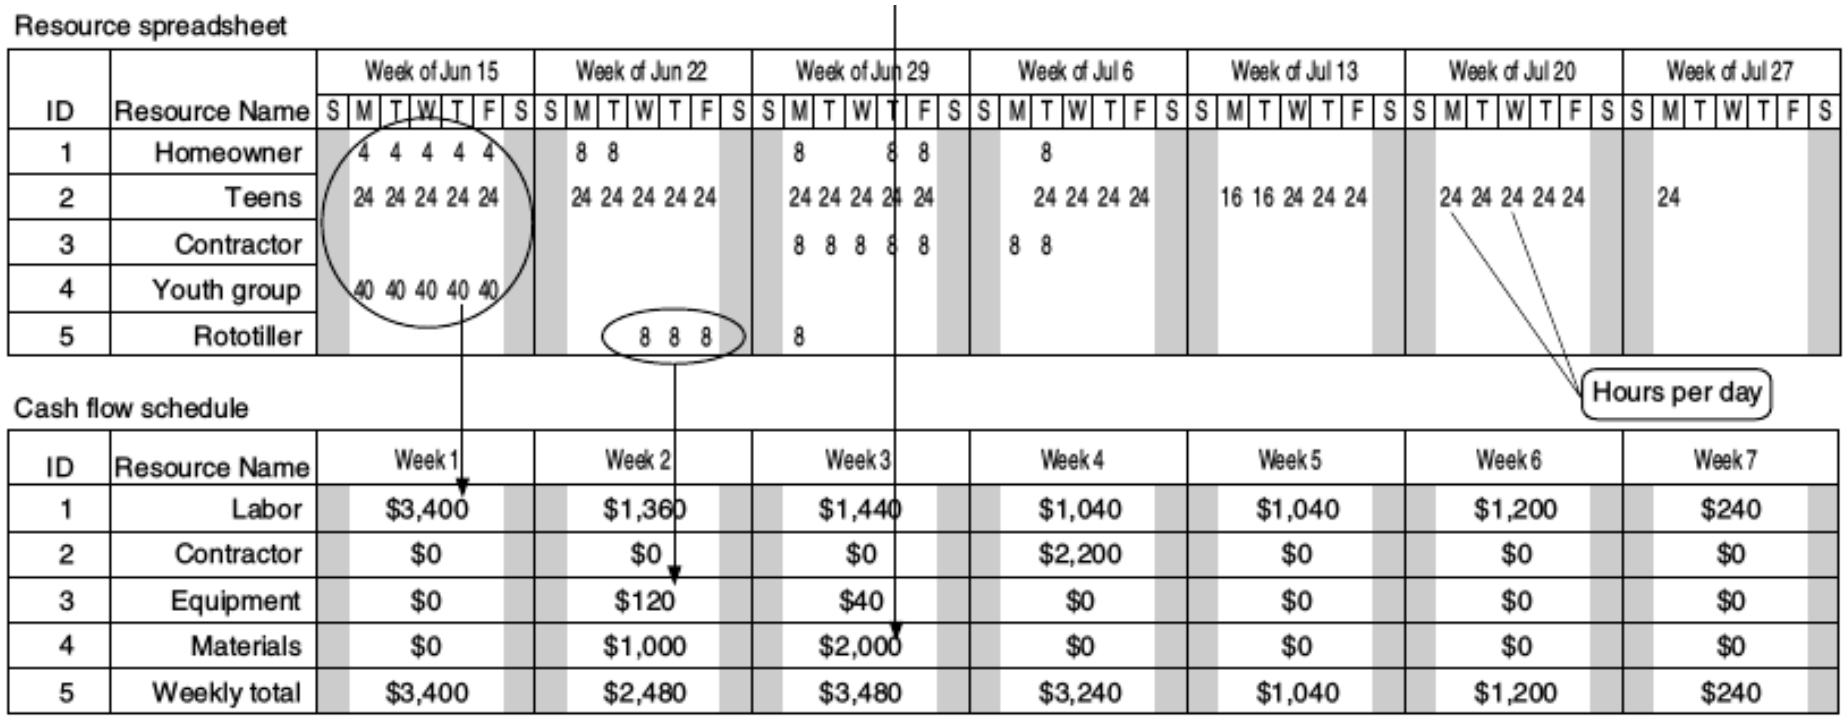
\includegraphics[width=0.95\textwidth]{cashFlow.png}
        \end{center}
    \end{frame}

    \section{Оценка}

    \begin{frame}
        \frametitle{Типичные ошибки при оценке проектов}
        \begin{itemize}
            \item Оценку делали не те люди
            \begin{itemize}
                \item Мало опыта, непонимание техник оценивания
            \end{itemize}
            \item Слишком быстрый ответ
            \begin{itemize}
                \item Оценка в условиях недостаточной информации
            \end{itemize}
            \item Забыли про риски и прочие буферы
            \item Забыли налоги
            \item Забыли про расходы на ``административный аппарат''
            \item Забыли про отпуск
            \item Забыли про индексацию зарплат
            \item Забыли про закупки
            \item Политика vs здравый смысл
        \end{itemize}
    \end{frame}

    \begin{frame}
        \frametitle{Уровни детальности оценки}
        \begin{itemize}
            \item ``Оценка в лифте''
            \item Оценка при выборе проекта
            \item Детальная оценка
        \end{itemize}
        \begin{center}
            
\includegraphics[width=0.7\textwidth]{dilbertEstimation.png}
        \end{center}
    \end{frame}

    \section{Отслеживание прогресса}

    \begin{frame}
        \frametitle{Деятельности по контролю за проектом, PMBOK}
        \begin{center}
            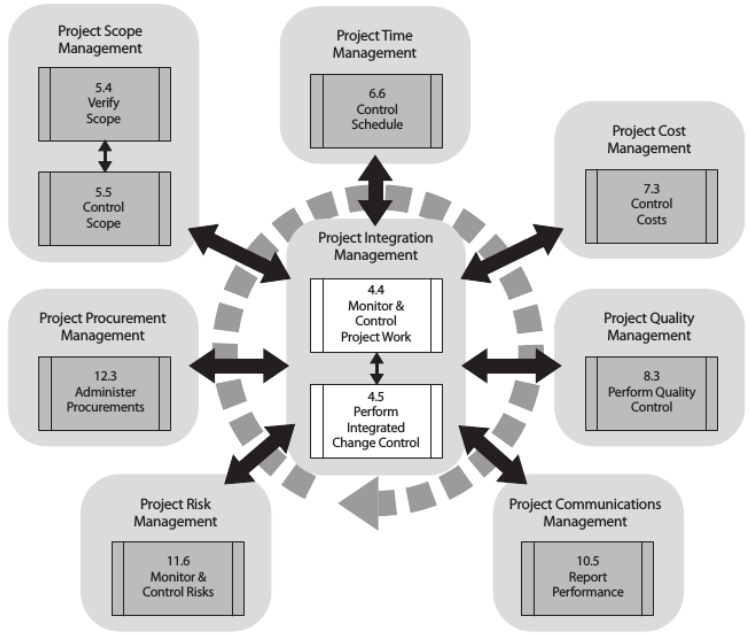
\includegraphics[width=0.6\textwidth]{pmbokProjectManagement.png}
        \end{center}
    \end{frame}

    \begin{frame}
        \frametitle{Треугольник равновесия}
        \begin{columns}
            \begin{column}{0.5\textwidth}
                \begin{center}
                    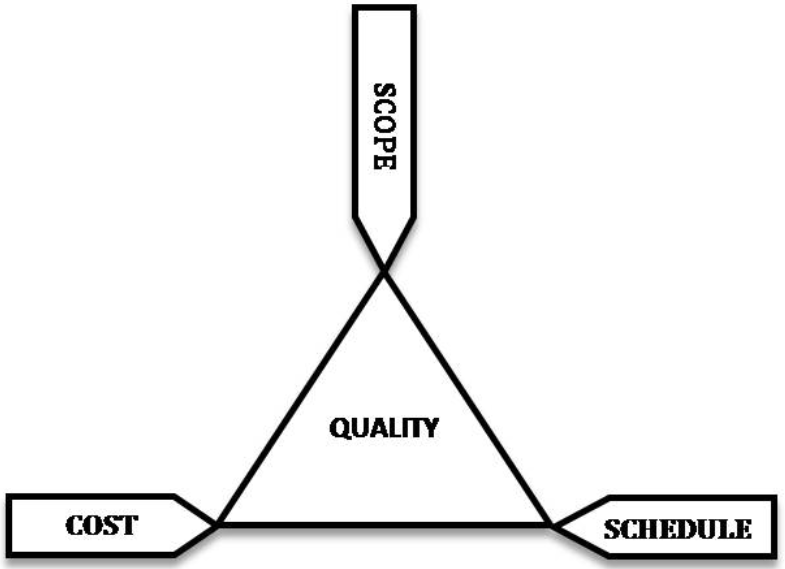
\includegraphics[width=0.9\textwidth]{balanceTriangle.png}
                \end{center}
            \end{column}
            \begin{column}{0.5\textwidth}
                \begin{center}
                    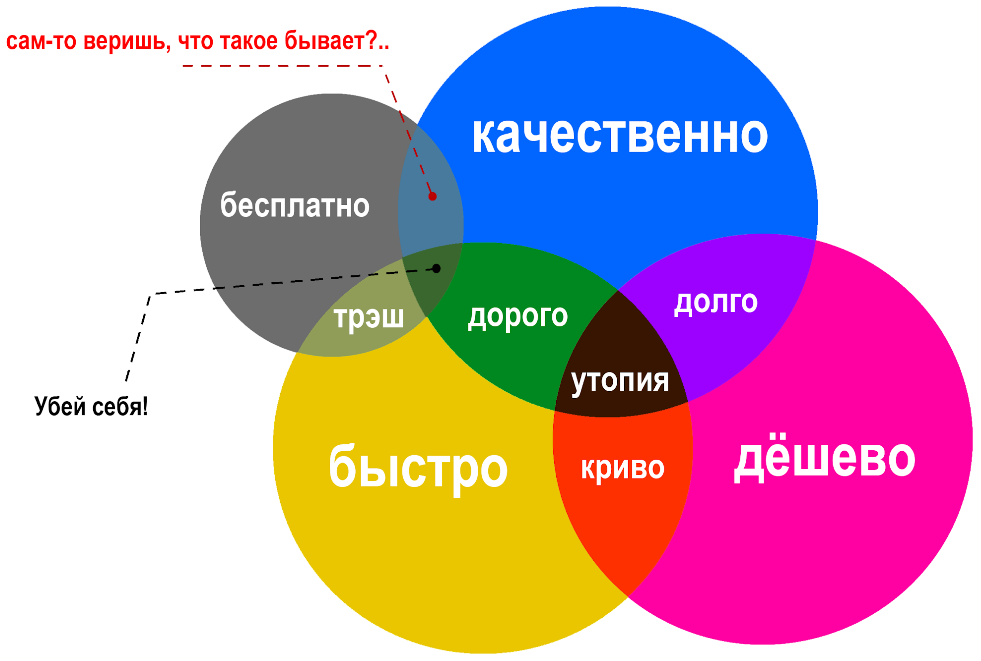
\includegraphics[width=0.9\textwidth]{balanceTriangleExplained.png}
                \end{center}
            \end{column}
        \end{columns}
    \end{frame}

    \begin{frame}
        \frametitle{Балансирование на уровне проекта}
        \begin{itemize}
            \item Повторная оценка задач
            \item Перераспределение задач критического пути
            \item Добавление людей в проект
            \item Привлечение экспертов
            \begin{itemize}
                \item Внутренние и внешние
                \item Создание экспертов внутри проекта
            \end{itemize}
            \item Аутсорсинг частей проекта
            \item Сверхурочная работа
            \item Снижение качества проекта
        \end{itemize}
    \end{frame}

    \begin{frame}
        \frametitle{Балансирование на уровне бизнес-целей}
        \begin{itemize}
            \item Изменение границ проекта
            \item Подстраивание проекта под дедлайны
            \item Работа на опережение
            \item Incremental delivery
            \item Создание прототипа
            \item Снижение прибыльности проекта
        \end{itemize}
    \end{frame}

    \begin{frame}
        \frametitle{Отслеживание прогресса проекта}
        \begin{itemize}
            \item Задачи
            \begin{itemize}
                \item Небольшой объём
                \item Чёткие критерии завершенности
                \item Регулярные обновления статуса
                \begin{itemize}
                    \item Правило 0-50-100
                \end{itemize}
            \end{itemize}
            \item Люди
            \begin{itemize}
                \item Регулярные (еженедельные) отчёты 
            \end{itemize}
            \item Дефекты
            \item Коммиты
            \item График
            \begin{itemize}
                \item Диаграмма Гантта
                \item Критический путь
                \item Измерение прогресса, а не затрат
            \end{itemize}
        \end{itemize}
    \end{frame}

    \begin{frame}
        \frametitle{Некоторые полезные показатели}
        \begin{itemize}
            \item Budgeted cost of work performed ($BCWP$)
            \item Actual cost of work performed ($ACWP$)
            \item Cost variance ($CV$) $= BCWP - ACWP$
            \item Cost variance percent ($CV\%$) $= CV / BCWP$
            \item Cost performance index ($CPI$) $= BCWP / ACWP$
            \item Budget at completion ($BAC$)
            \item Estimate budget at completion ($EAC$) $= BAC / CPI$
        \end{itemize}
    \end{frame}

    \begin{frame}
        \begin{center}
            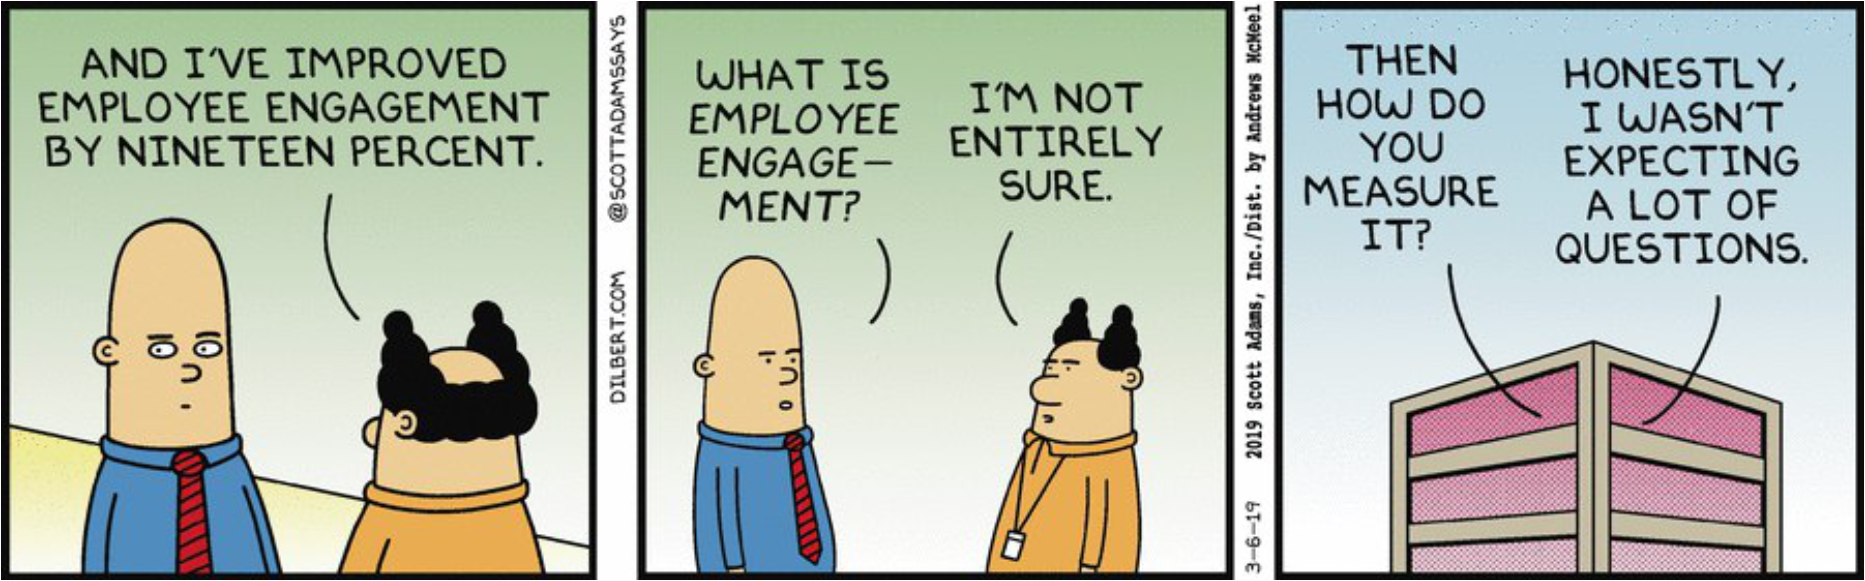
\includegraphics[width=0.9\textwidth]{dilbertEmployeeEngagement.png}
        \end{center}
    \end{frame}

    \begin{frame}
        \frametitle{Отслеживание затрат и времени}
        \begin{center}
            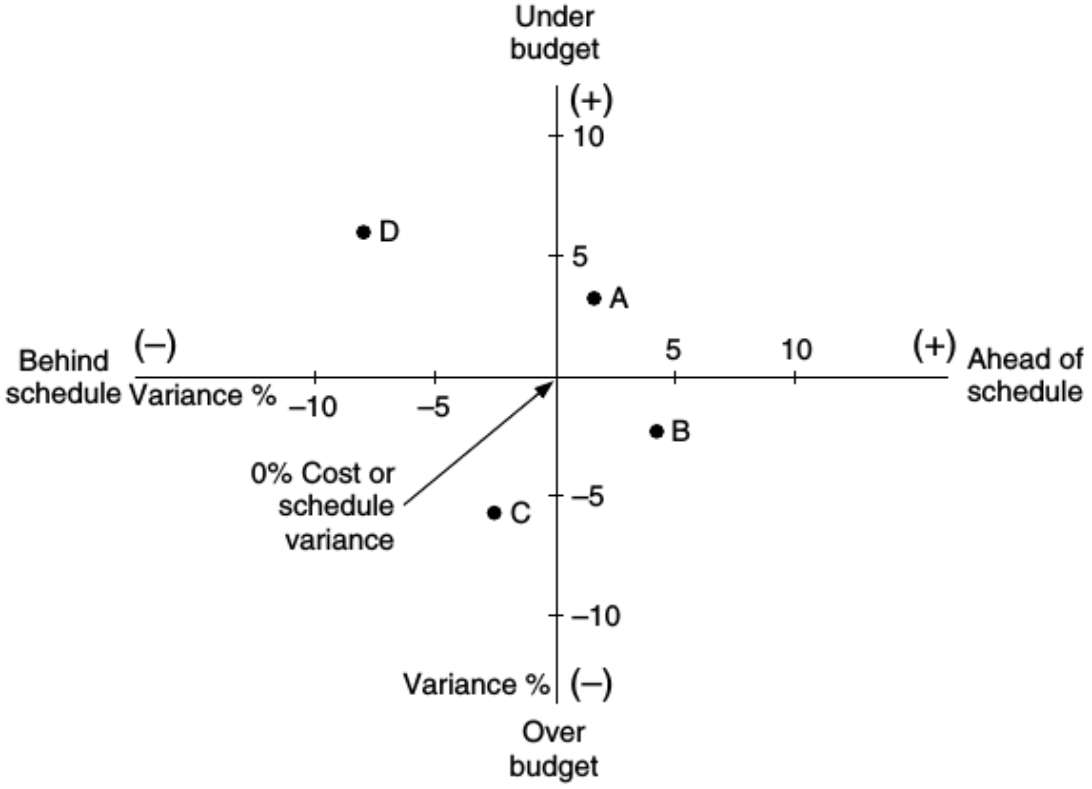
\includegraphics[width=0.8\textwidth]{varianceGraph.png}
        \end{center}
    \end{frame}

    \begin{frame}
        \frametitle{Прогресс работ и метрики}
        \begin{center}
            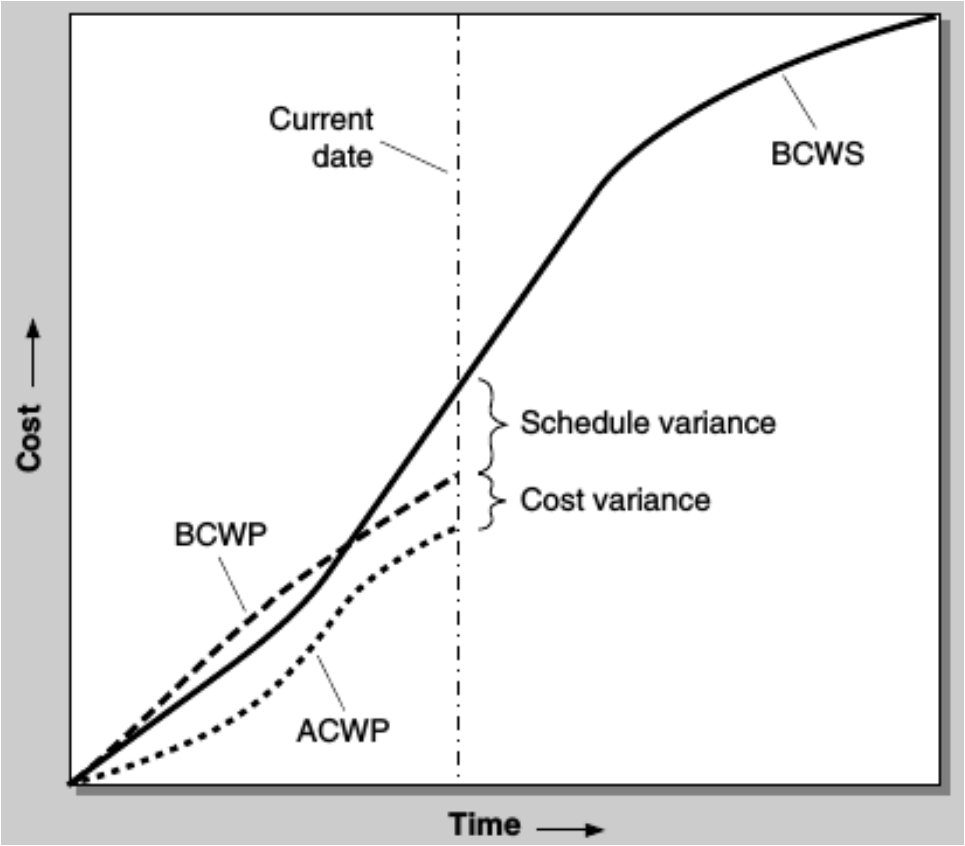
\includegraphics[width=0.6\textwidth]{metricsGraph.png}
        \end{center}
    \end{frame}

    \begin{frame}
        \frametitle{Пороги эскалации}
        \begin{center}
            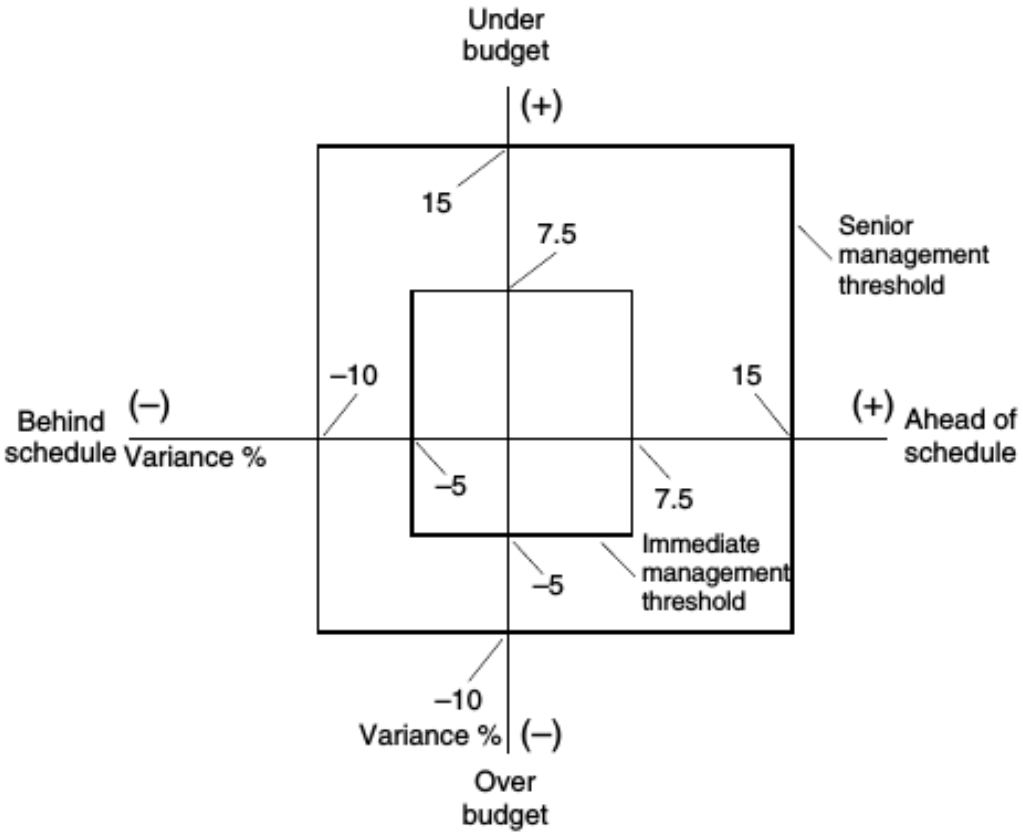
\includegraphics[width=0.7\textwidth]{escalationThresholds.png}
        \end{center}
    \end{frame}

\end{document}
